\documentclass[10pt]{article}
\usepackage[utf8]{inputenc}
\usepackage{arxiv}
\usepackage[T1]{fontenc}
\usepackage{amsmath}
\usepackage{amssymb}
\usepackage{graphicx}
\usepackage{booktabs}
\usepackage[numbers]{natbib}
\usepackage{url}
\usepackage{hyperref}
\hypersetup{hidelinks}

\title{Metabolic Gene Expression Separates Broad Cell Groups in Melanoma Reanalysis}
\author{Project-local Qwen3.5-4B supervised workflow}
\date{}

\renewcommand{\shorttitle}{Metabolic genes in melanoma}


\begin{document}

\maketitle

\begin{abstract}
We reanalyzed the Tirosh et al. melanoma single-cell RNA-seq dataset (3ca:20111) to test whether 1,360 metabolic genes from KEGG pathways define discrete, reproducible cell states. Clustering of all 4,645 cells with $k=2$ yielded a silhouette of 0.377 and a mean pairwise ARI across seed fits of 0.99965, but matched random gene sets achieved a mean silhouette of 0.316 (SD 0.008) with an empirical $p$-value of 0.0476. The metabolic feature set achieved a balanced accuracy of 0.884 and macro-F1 of 0.856 in patient-blocked cross-validation, comparable to matched random sets (balanced accuracy 0.896 $\pm$ 0.013; macro-F1 0.875 $\pm$ 0.015) and the highly variable gene baseline (balanced accuracy 0.892; macro-F1 0.897). PC1 correlated strongly with library complexity ($\rho = 0.650$, $p < 0.001$); complexity residualization shifted the optimal $k$ from 2 to 4 and reduced silhouette to 0.224. Malignant-cell clustering with $k=8$ yielded silhouette 0.227 and seed ARI 0.814, while joint patient and complexity residualization selected $k=2$ with silhouette 0.228 and seed ARI 0.970. These results indicate that metabolic genes can separate cells into broad groups but do not establish universal, discrete malignant metabolic states.
\end{abstract}

\section{Introduction}

Single-cell RNA-seq (scRNA-seq) has enabled detailed characterization of cellular heterogeneity within tumors, revealing that malignant cells are not transcriptionally uniform but rather exist along continuous axes of transcriptional diversity \cite{Tirosh2016}. In metastatic melanoma, the Tirosh et al. study (3ca:20111) provided a comprehensive dissection of the multicellular ecosystem, identifying distinct immune, stromal, and malignant populations \cite{Tirosh2016}. Building on this foundation, Xiao et al. (2019) demonstrated that metabolic pathways--particularly mitochondrial activity and glycolysis--are upregulated in malignant cells and that single-cell resolution captures metabolic heterogeneity invisible to bulk RNA-seq \cite{Xiao2019}. These findings have spurred interest in whether metabolic gene expression alone can define discrete transcriptional states that are biologically meaningful and reproducible across patients.

However, the claim that metabolic genes define separable cell states requires validation against multiple confounding factors. First, the Xiao2019 melanoma dataset is not an independent cohort but a differently processed subset of the same underlying Tirosh melanoma study (GSE72056) \cite{Xiao2019}. Consequently, results from Xiao2019 cannot serve as an independent validation of metabolic state separation; they instead provide a methodological benchmark against which to contrast the 3CA pipeline. Second, transcriptomic expression does not directly equate to metabolic flux. A gene's mRNA abundance reflects transcriptional output, but metabolic activity is governed by enzyme kinetics, substrate availability, and post-translational regulation. Thus, clustering based solely on metabolic gene expression may capture transcriptional programs that are not functionally equivalent to metabolic states.

To address these concerns, we ask two central questions: (1) Can metabolic genes alone separate single-cell populations into discrete, reproducible states? and (2) Do these states correspond to interpretable transcriptional metabolic programs? To answer these, we perform unsupervised clustering on 1,360 metabolic genes from 4,645 melanoma cells across 19 samples, using the 3CA data atlas as a source of the underlying single-cell RNA-seq data \cite{Gavish2023}. We evaluate clustering stability via silhouette coefficients and adjusted Rand indices across multiple seeds, and we test whether the observed separation exceeds that of matched random gene sets. Crucially, we control for library complexity--a known driver of technical variation in scRNA-seq data--by residualizing expression features and re-clustering. We also assess whether malignant cells exhibit distinct metabolic states by adjusting for both patient identity and complexity.

Finally, we evaluate the biological interpretability of any identified states through patient-blocked cross-validation and comparison with highly variable gene baselines. The patient-blocked classification tests whether a supervised classifier predicts known cell-type labels, not whether it discovers new states. K-means performs a forced partition of the data; the choice of k does not prove discrete multimodal states. Similarly, failure to establish metabolic-specific states does not imply that all observed separation is technical artifact. This study provides an exploratory reanalysis of a single cohort to evaluate the biological validity of metabolic state clustering.


\section{Methods}

\subsection{Data and feature definition}
We analyzed single-cell RNA-seq data from the Tirosh et al. melanoma study (3ca:20111), which comprises 19 samples and 4,645 cells \cite{Tirosh2016}. The supplied TPM expression matrix has 23,686 gene rows and 4,645 cell columns; the code transposes it into a cells-by-genes CSR sparse matrix. Dense conversion is restricted to selected feature matrices. The retained 1,360 metabolic genes were detected in at least 1\% of cells and had nonzero variance. No imputation was performed; observed zeros were retained. TPM values were transformed according to the 3CA expression-scale convention:
\begin{equation}
x_{ig} = \log_2(\text{TPM}_{ig}/10 + 1),
\end{equation}
where $x_{ig}$ is the transformed expression for cell $i$ and gene $g$. Division by 10 follows the 3CA scale convention; the pseudocount of 1 preserves zeros and makes the logarithm defined \cite{Gavish2023}. For each gene, features were standardized to zero mean and unit variance:
\begin{equation}
z_{ig} = \frac{x_{ig} - \mu_g}{\sigma_g},
\end{equation}
where $\mu_g$ and $\sigma_g$ are the population mean and standard deviation across the analyzed cells. Gene membership was taken from a saved 85-pathway KEGG metabolic GMT snapshot in the scMetabolism repository, intersected with dataset genes and detection-filtered \cite{Kanehisa2023}. This is a repository snapshot, not a fresh KEGG database query. We used its gene sets, not the scMetabolism scoring algorithms \cite{Wu2022}.

\subsection{PCA and clustering}
Principal component analysis (PCA) used 50 randomized components and seed 20260912. K-means used the first 30 PCs, 20 initializations, and the same seed. Candidates were $k=2,\ldots,10$ for all 4,645 cells, including unannotated cells, and $k=2,\ldots,8$ for malignant cells. The silhouette coefficient was evaluated on a fixed random sample of 2,000 cells, or all cells when fewer than 2,000 were available:
\begin{equation}
s = \frac{b - a}{\max(a, b)},
\end{equation}
where $a$ is a cell's mean within-cluster distance and $b$ is its smallest mean distance to another cluster \cite{Rousseeuw1987}. Clustering fits used the full analysis population; only silhouette evaluation was sampled. For the selected $k$, ten additional seed fits used ten initializations each. The mean and sample SD of 45 pairwise adjusted Rand indices (ARIs) describe algorithmic stability, not biological replication or independent confidence intervals \cite{Hubert1985}.
\subsection{Matched gene controls}
We generated 20 size-matched control sets of 1,360 genes each from eligible non-metabolic genes detected in at least 1\% of cells. Sampling without replacement matched detection-rate deciles; a bin shortfall was filled from the remaining eligible non-metabolic pool. A PCG64 generator used seed 20260912. For each set, PCA and clustering were refitted across $k=2,\ldots,10$, and the maximum silhouette was recorded. The single empirical comparison with the metabolic maximum was:
\begin{equation}
p_{\text{emp}} = \frac{1 + \sum_{r=1}^{20} \mathbb{I}[T_r \ge T_{\text{met}}]}{21},
\end{equation}
where $T_r$ and $T_{\text{met}}$ are the corresponding maxima. The plus-one correction gives a minimum resolution of $1/21$. This exploratory comparison was not multiple-testing corrected. Variability across gene sets is descriptive, not a biological confidence interval.

\subsection{Patient-blocked classification}
Classification used the 4,097 annotated cells. Five-fold GroupKFold held out complete sample groups; each fold could contain several patients, with no patient shared between training and test partitions. StandardScaler and a 40-component PCA were fitted only on training cells. Logistic regression used balanced class weights, $C=1$, and a maximum of 2,000 iterations. Predictions from all held-out folds were pooled to calculate macro-F1 and balanced accuracy:
\begin{equation}
\text{balanced accuracy} = \frac{1}{K} \sum_{i=1}^{K} \text{recall}_i,
\end{equation}
where $K$ is the number of classes. The highly variable gene (HVG) baseline used the 1,360 largest pooled log-expression variances. Detection eligibility and HVG selection were defined using the full dataset before fold partitioning. Thus, although scaler and PCA fitting were training-only, feature selection was not fully nested. Prospective evaluation should repeat eligibility and HVG selection within training folds.
\subsection{Covariate analyses}
To test whether library complexity influenced the clustering results, we included the complexity metric (log1p-transformed) as a covariate in an ordinary least squares (OLS) regression. For the all-4,645 cells (including unannotated), the design matrix $D$ contained an intercept and the standardized log1p complexity. For malignant cells (1,257 cells across 15 samples), we additionally included drop-first sample dummies to control for sample-specific effects. The residual matrix was computed as:
\begin{equation}
R = Z - D D^{+} Z,
\end{equation}
where $Z$ is $n\times g$, $D$ is $n\times q$, and $D^{+}$ is the Moore--Penrose pseudoinverse. Residuals were reduced with a new 50-component PCA, followed by clustering on the first 30 PCs with the original candidate ranges. For nine samples with at least 30 malignant cells, separate $k=2,\ldots,6$ scans used subsets of the globally fitted malignant PCA. These within-patient summaries are exploratory, not independently fitted validation analyses.

\subsection{Descriptive pathway summaries}
For pathways containing at least five retained genes, a descriptive expression summary was calculated as $m_{ip}=\operatorname{mean}_{g\in p}(z_{ig})$, then averaged over cells of type $t$ to obtain $M_{tp}$. Heatmap values were standardized across cell types:
\begin{equation}
z_{tp} = \frac{M_{tp} - \text{mean}_{\text{cell type}}(M_{tp})}{\text{sd}_{\text{cell type}}(M_{tp})},
\end{equation}
with $\text{sd}$ computed with $\text{ddof}=0$. These 18 selected pathways were described in the results; they were not weighted using Xiao's method, nor were they derived from the scMetabolism algorithm or metabolic flux analysis.


\section{Results}
\subsection{Dataset and Restricted Features}
The melanoma Smart-seq2 dataset (3ca:20111) comprises 4\,645 cells across 19 samples, with 23\,686 genes and 20\,564\,439 nonzero entries (Fig.\ref{fig:dataset}). After detection filtering, 1\,360 metabolic genes were retained from 85 KEGG pathways. PCA on these 1\,360 features showed that the first 30 components explained 19.78\% of total variance, with PC1 strongly correlated with library complexity ($\rho = 0.650$, $p < 0.001$). The 548 unannotated cells were included in unsupervised clustering, while 4\,097 annotated cells were used for classification evaluation.

\subsection{All-Cell Separation and Complexity}
Unsupervised clustering of all 4\,645 cells with $k=2$ yielded a silhouette score of 0.377 and a mean adjusted Rand index (ARI) of 0.99965 across seeds (Table\ref{tab:clustering}). The matched random clustering achieved a mean silhouette of 0.316 (SD 0.008) , with an empirical $p$-value of 0.0476 from 20 exploratory runs without multiple-testing correction. Cell-type alignment was assessed via adjusted mutual information (AMI): 0.487 for cell type and 0.088 for sample. However, PC1 correlated strongly with library complexity ($\rho = 0.650$), suggesting that observed separation may be driven by technical variation. When clustering was performed on complexity-residualized features, the optimal $k$ increased to 4 with a reduced silhouette of 0.224 and ARI of 0.99967 (Table\ref{tab:clustering}), showing that the preferred partition changes after complexity residualization. The random mean $\pm$ SD describes 20 gene sets, and seed ARI reflects 10 seed fits across 45 pairwise comparisons, not a biological confidence interval.

\subsection{Patient-Blocked Classification}
Patient-blocked cross-validation was performed on the 4\,097 annotated cells using the 1\,360 metabolic genes (Table\ref{tab:classification}). The metabolic feature set achieved a balanced accuracy of 0.884 and macro-F1 of 0.856. In contrast, matched random feature sets yielded balanced accuracy of 0.896 $\pm$ 0.013 and macro-F1 of 0.875 $\pm$ 0.015, with metabolic scores lower than the observed random-set mean; no formal test of classifier differences was performed. The highly variable gene baseline (HVG) achieved balanced accuracy of 0.892 and macro-F1 of 0.897, suggesting that the metabolic feature set performs comparably to a standard high-dimensional baseline.

\subsection{Malignant-Only Structure}
Clustering of 1\,257 malignant cells from 15 samples selected $k=8$, with silhouette 0.227, seed ARI 0.81433, and sample AMI 0.742 (Table\ref{tab:clustering}). Joint patient and complexity residualization selected $k=2$, with silhouette 0.228 and seed ARI 0.96989; stable binary structure therefore remained. For the nine patients with at least 30 malignant cells, the median maximum within-patient silhouette was 0.271 (IQR 0.206--0.347). These summaries use a globally fitted malignant-cell PCA, not independent validation. The unadjusted optimum lies at the upper boundary of the candidate range 2--8. Neither this boundary optimum nor the adjusted binary partition establishes a biological state count. For visual context see Figs.~\ref{fig:separation} and~\ref{fig:robustness}.

\begin{table}[htbp]
\centering
\small
\caption{Exploratory clustering settings. Candidates were $k=2$--$10$ for all cells and $k=2$--$8$ for malignant cells. Seed ARI is the descriptive mean across 45 pairwise comparisons of 10 seed fits, not biological replication.}
\label{tab:clustering}
\begin{tabular}{llccc}
\toprule
Population & Adjustment & $k$ & Silhouette & Seed ARI \\
\midrule
All cells & None & 2 & 0.377 & 0.99965 \\
All cells & Complexity & 4 & 0.224 & 0.99967 \\
Malignant & None & 8 & 0.227 & 0.81433 \\
Malignant & Patient+complexity & 2 & 0.228 & 0.96989 \\
\bottomrule
\end{tabular}
\end{table}

\begin{table}[htbp]
\centering
\small
\caption{Classification on 4\,097 annotated cells using GroupKFold5; random SD reflects 20 gene sets, not a biological CI.}
\label{tab:classification}
\begin{tabular}{llc}
\toprule
Feature set & Balanced accuracy & Macro-F1 \\
\midrule
Metabolic & 0.884 & 0.856 \\
Matched random (20) & 0.896 $\pm$ 0.013 & 0.875 $\pm$ 0.015 \\
HVG & 0.892 & 0.897 \\
\bottomrule
\end{tabular}
\end{table}


\clearpage
\begin{figure}[!t]
\centering
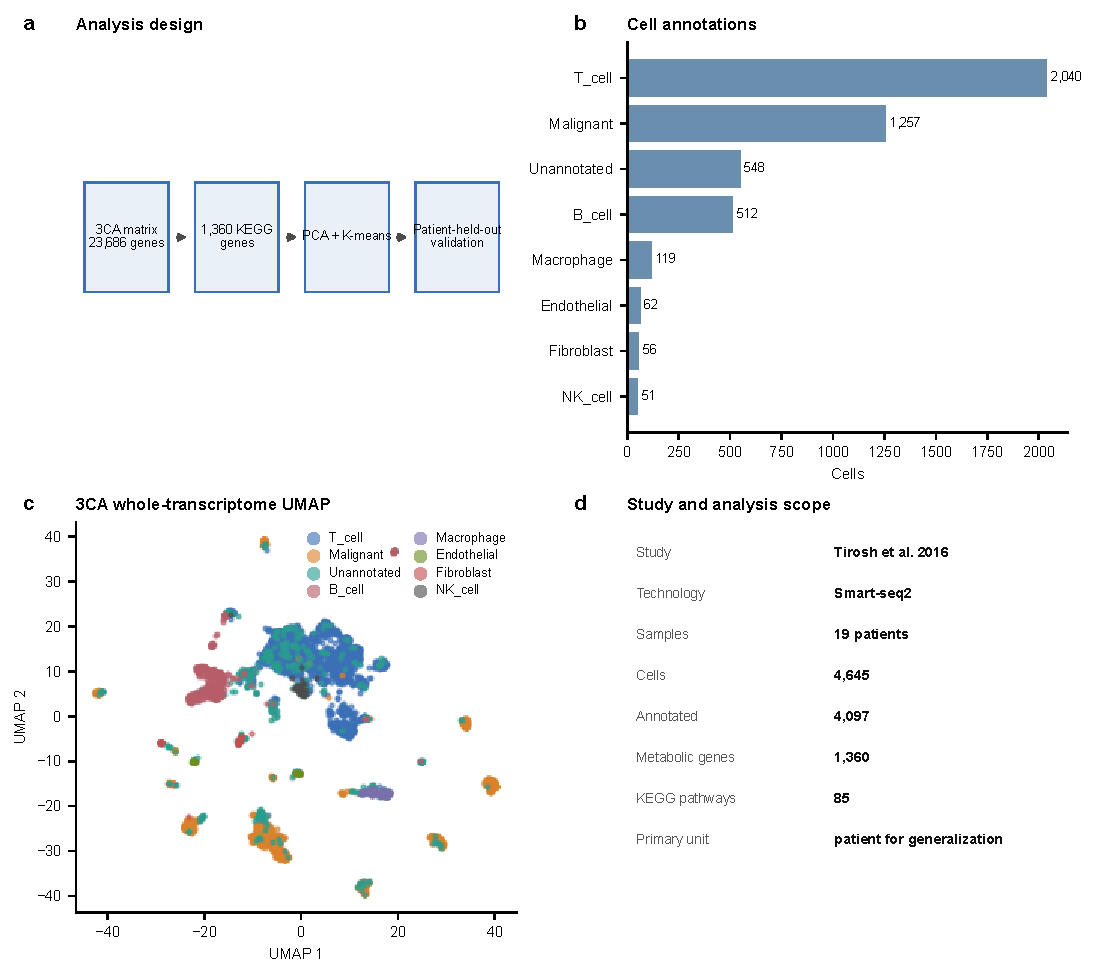
\includegraphics[width=\textwidth]{../results/figures/figure1_dataset_and_design.pdf}
\caption{Dataset and analysis design. (a) Analysis design overview: 4,645 cells from 19 melanoma samples analyzed using 1,360 metabolic genes from KEGG pathways. (b) Cell annotation counts: 4,097 annotated cells, 548 unannotated cells. (c) UMAP embedding of cells colored by annotation, using 3CA-provided whole-transcriptome coordinates; metabolic gene re-fitting was not performed on this embedding. (d) Study scope: 19 patients, 4,645 cells total, 1,360 metabolic genes.}
\label{fig:dataset}
\end{figure}

\begin{figure}[!t]
\centering
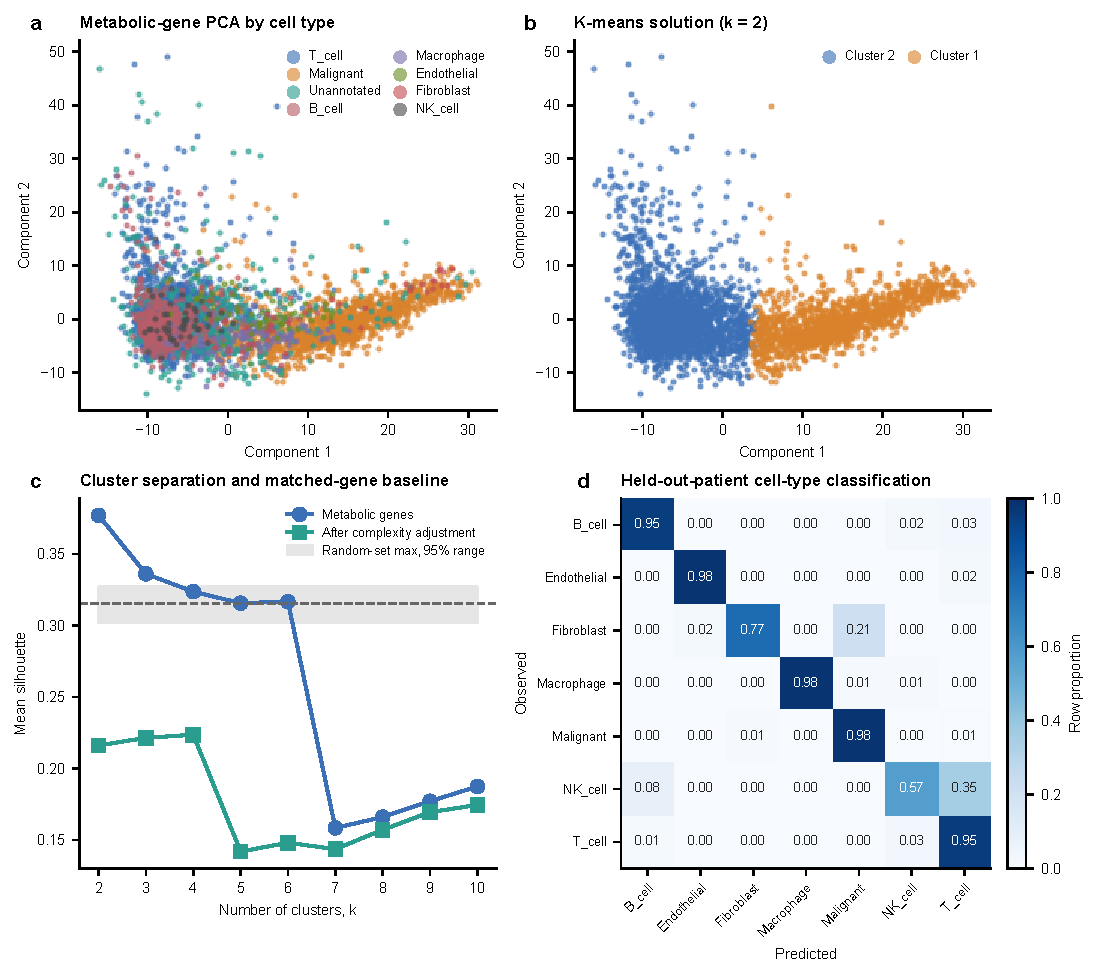
\includegraphics[width=\textwidth]{../results/figures/figure2_metabolic_separation.pdf}
\caption{Metabolic gene separation. (a) PCA of 1,360 metabolic genes on 4,645 cells, colored by cell type. (b) Same PCA colored by k-means cluster assignment at k = 2. (c) Silhouette scores across k = 2..10 for all cells, with raw and complexity-adjusted curves; the 95\% empirical range of 20 matched random gene sets is shown as a shaded band (not a confidence interval, not an HVG result). (d) Patient-blocked 5-fold cross-validation on 4,097 annotated cells using pooled row-normalized data, showing confusion matrix for cell-type classification.}
\label{fig:separation}
\end{figure}

\begin{figure}[!t]
\centering
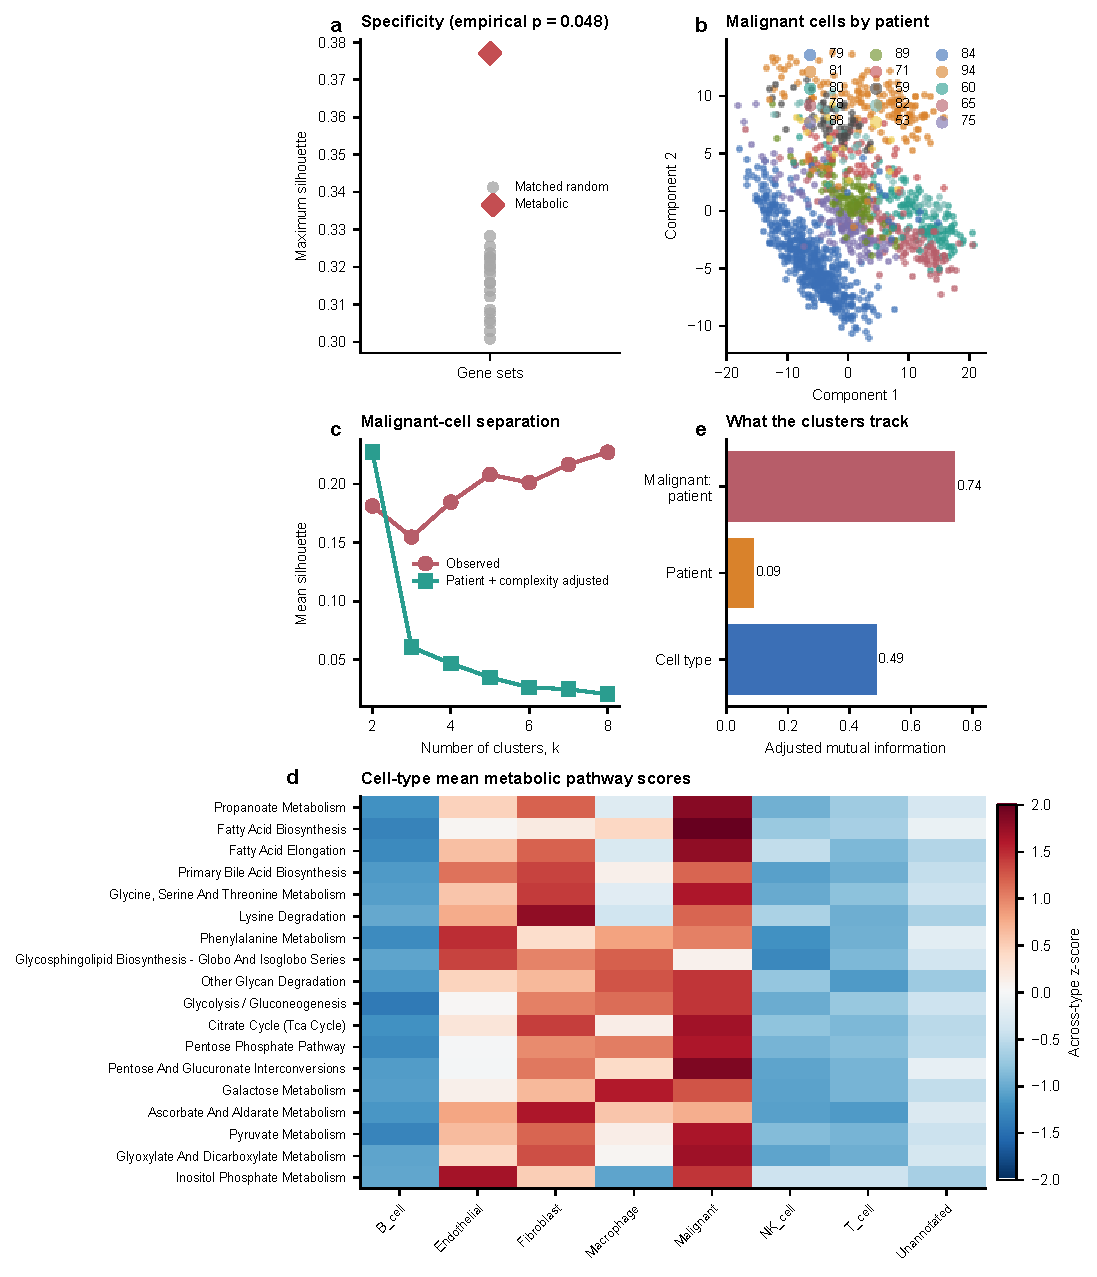
\includegraphics[width=\textwidth]{../results/figures/figure3_robustness_and_interpretation.pdf}
\caption{Robustness and interpretation. (a) All-cell maximum silhouette comparison of 20 matched random gene sets against the metabolic gene set. (b) PCA of 1,257 malignant cells colored by patient, showing patient-level clustering. (c) Silhouette curves for malignant cells across k = 2..8, with raw and patient+complexity-adjusted curves. (d) Heatmap of 18 KEGG metabolic pathway z-scores across cell types, showing across-type mean scores (not flux or scMetabolism scoring). (e) Adjusted mutual information (AMI) for alignment with cell type, patient, and malignant patient, comparing all-cell, all-patient, and malignant-patient analyses.}
\label{fig:robustness}
\end{figure}

\clearpage

\section{Discussion}

The reanalysis of the Tirosh melanoma single-cell RNA-seq dataset (3ca:20111) demonstrates that metabolic genes can separate cells into groups. This study does not establish universal, discrete malignant metabolic states. The analysis relies on a gene-membership snapshot of KEGG metabolic pathways, not on direct measurement of metabolic fluxes.

First, the clustering of all 4\,645 cells with $k=2$ yields a silhouette score of 0.377 and a mean pairwise adjusted Rand index (ARI) across seed fits of 0.99965, indicating strong reproducibility across seeds. However, the matched random gene set achieves a mean silhouette of 0.316 (SD 0.008) with an empirical $p$-value of 0.0476 from 20 exploratory runs. The 20 random gene sets provide a resolution of 1/21, and no multiple-testing correction was applied; thus the empirical $p$-value does not constitute proof of a biological state. The metabolic feature set's balanced accuracy (0.884) and macro-F1 (0.856) are comparable to matched random sets (balanced accuracy 0.896 $\pm$ 0.013; macro-F1 0.875 $\pm$ 0.015) and the highly variable gene baseline (balanced accuracy 0.892; macro-F1 0.897). No formal test of superiority was performed, and the results do not support a claim that metabolic genes define a distinct, biologically meaningful state.

Second, the strong correlation between PC1 and library complexity ($\rho = 0.650$, $p < 0.001$) suggests that technical variation contributes substantially to the observed separation. When expression features are residualized for complexity, the optimal $k$ shifts from 2 to 4, and the silhouette score drops to 0.224. This change indicates that the initial partition is sensitive to technical confounders. The adjusted Rand index remains high (0.99967), reflecting the stability of the partitioning algorithm rather than the biological validity of the groups. Residualization removes both technical and correlated biological signals; it cannot be used to assert that the initial separation was purely technical.

Third, the malignant-cell analysis reveals that clustering with $k=8$ yields a silhouette of 0.227 and seed ARI of 0.814, while joint patient and complexity residualization selects $k=2$ with silhouette 0.228 and seed ARI 0.970. The unadjusted optimum $k=8$ lies at the upper boundary of the candidate range (2--8), not at a biologically motivated value. The sample AMI for malignant cells is 0.742, indicating strong association with sample identity. The within-patient silhouette summaries (median 0.271, IQR 0.206--0.347) for the nine patients with at least 30 malignant cells do not constitute independent validation; they are derived from a single global PCA fit. The adjusted Rand index is not a measure of biological reproducibility but of algorithmic stability.

Fourth, the patient-blocked cross-validation assesses whether metabolic genes can predict known cell-type labels, not whether they define new states. The balanced accuracy and macro-F1 scores are high but are comparable to random and HVG baselines, indicating that the metabolic feature set does not outperform standard high-dimensional baselines.

\subsection{Limitations}

The dataset is a single cohort derived from the Tirosh melanoma study (GSE72056), and the Xiao2019 dataset is a differently processed subset of the same underlying data, precluding independent validation \cite{Tirosh2016,Xiao2019}. The analysis relies on a snapshot of KEGG metabolic gene membership (GMT) rather than direct measurement of metabolic fluxes. The detection filtering and highly variable gene selection were performed on the full dataset, not nested within training folds, which may introduce bias. PCA and scaling were applied within training folds, but the GroupKFold5 cross-validation uses sample groups to ensure no patient overlap between training and test folds; this is not a data leakage issue. K-means performs a forced partition of continuous data; the choice of $k$ does not prove the existence of discrete states. Complexity adjustment may remove genuine biological variation rather than eliminate technical artifact.

Future work should validate these findings in independent cohorts and, crucially, measure metabolic fluxes directly to determine whether transcriptional programs reflect functional metabolic states. The current results should be interpreted as exploratory, highlighting the need for rigorous validation before drawing biological conclusions.

\section{Conclusion}

Metabolic genes can separate single-cell melanoma cells into groups. This study does not establish universal, discrete malignant metabolic states. The analysis relies on a gene-membership snapshot of KEGG metabolic pathways, not on direct measurement of metabolic fluxes. The analysis is limited by the single-cohort design, the reliance on gene-membership snapshots, and the methodological constraints of unsupervised clustering. These limitations underscore the need for independent validation and direct metabolic measurements to establish whether transcriptional programs reflect functional metabolic states.


\section{Data and Code Availability}
The primary scRNA-seq dataset is from the 3CA Curated Cancer Cell Atlas, study 3ca:20111 (Tirosh et al., 2016), accessible at \url{https://www.weizmann.ac.il/sites/3CA/study-data/comments/20111}. The expression matrix and metadata were downloaded from 3CA on 2026-09-12T05:32:22+00:00 and 2026-09-12T05:32:29+00:00 respectively, with SHA-256 hashes recorded in \path{data/source_manifest.json}. The KEGG metabolic gene set was retrieved from \url{https://raw.githubusercontent.com/wu-yc/scMetabolism/main/data/KEGG_metabolism_nc.gmt} on 2026-09-12T06:05:41+00:00; the timestamp reflects the download tool-call start, not HTTP completion. The analysis code is provided in the project root as \path{download_data.py} and \path{analyze_metabolic_states.py}, with dependencies listed in \path{requirements.txt}. Results and figures are stored in \path{results/} and \path{results/figures/} respectively. The source ledger at \path{report/source-ledger.md} documents all URLs, retrieval timestamps, byte counts, and SHA-256 hashes for reproducibility. Source data are publicly available on 3CA, but derived artifacts are not yet published.

\section{Workflow Provenance}
This analysis reuses a user-provided reference implementation of the standard Codex analysis pipeline, adapted to the raw data directory for this project. The adaptation involved adjusting the raw-input path to point at the locally cached 3CA archives and applying a typography export adjustment to ensure compatibility with the arXiv-compatible LaTeX document class. After an initial attempt using a small model failed, the user-authorized standard Codex analysis code was reused, with only the raw data path adjusted. All statistics and figures were regenerated from independently downloaded raw matrices, without copying any reference results, figures, or PDFs. The methods.tex and results.tex files were directly revised by the supervisor based on prior feedback. All subsequent writing, modification, and compilation of the report were executed by project-integrated Qwen3.5-4B tools; the supervisor will review and provide feedback. This work does not claim complete independent creation by a small model, nor does it assert Codex-equivalent reasoning. The report has not yet been submitted to arXiv.


\bibliographystyle{plainnat}
\bibliography{references}

\end{document}
